\section{Análisis de los resultados}
A continuación se muestran capturas del funcionamiento del código implementado.

\begin{figure}[H]
    \centering
    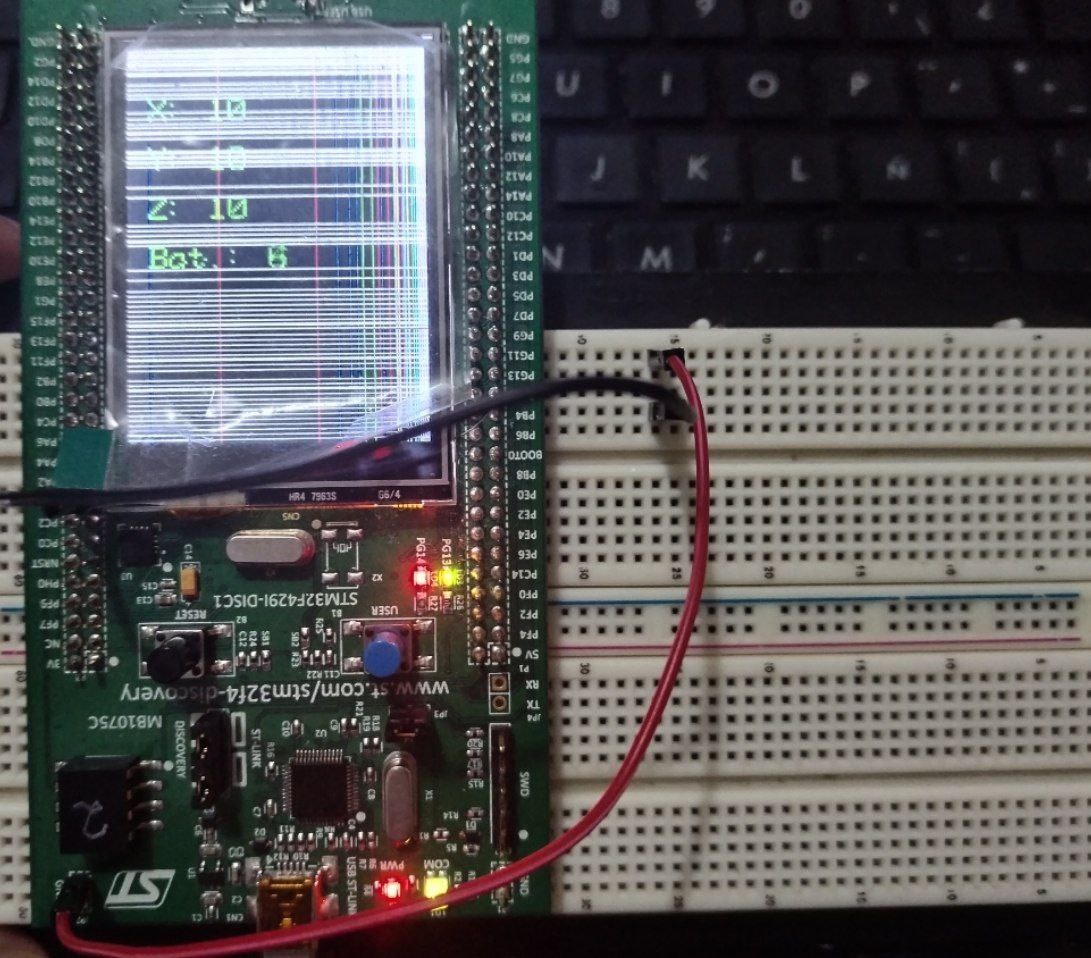
\includegraphics[scale=.3]{Imagenes/codig4.png}
    \caption{Muestra de información en pantalla.}
    \label{codig4}
\end{figure}

En la figura \ref{codig4} se muestra el funcionamiento de la placa, se pueden observar las siguientes características:
\begin{itemize}
    \item En pantalla se muestra el valor del giroscopio (simulado) en los tres ejes. No es claramente visible debido al daño que presenta la pantalla.
    \item Se muestra encendido el led verde, este indica que la comunicación USART se encuentra activa. Cuando se presiona el botón la comunicación se desactiva y el led se apaga.
    \item  Se puede observar el led rojo encendido. Este led parpadea indicando que la batería tiene un nivel de tensión inferior a 7.5V, esto también se puede observar en la pantalla, que indica una medida de 5mV, casi cero. esto porque el pin ADC se conectó con jumpers al pin GND. Si este pin se conecta a tensión, el valor en pantalla indica 9000mV, es decir, indica que la batería está cargada y por lo tanto el led rojo deja de parpadear.
\end{itemize}
\begin{figure}[H]
    \centering
    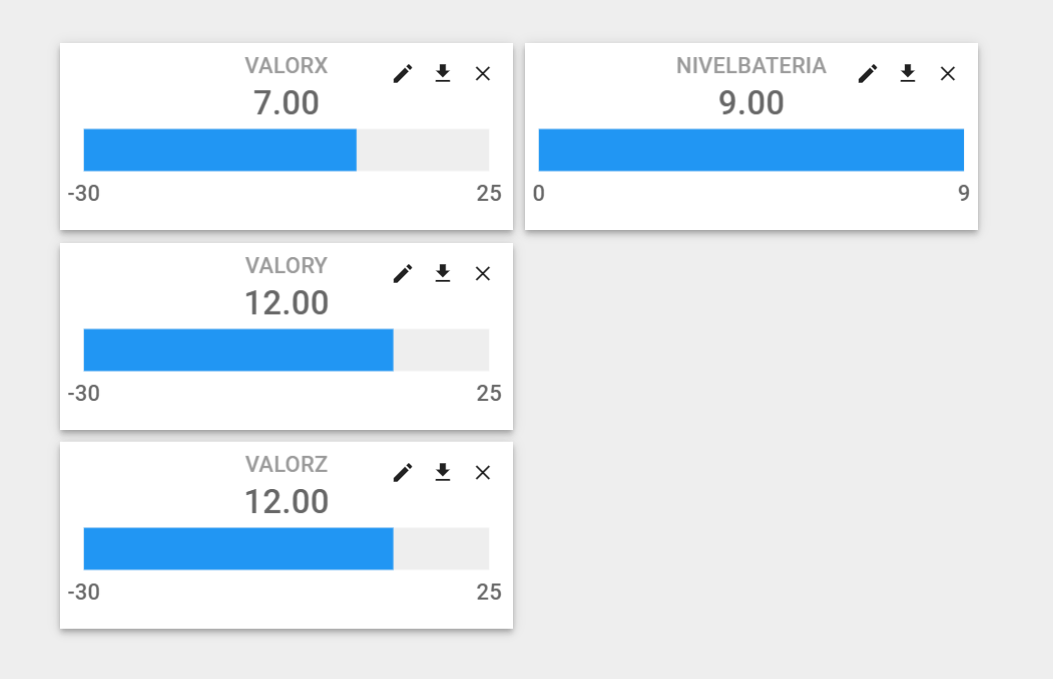
\includegraphics[scale=.3]{Imagenes/TB.png}
    \caption{Muestra del dashboard en thingsboard al que se conecta la placa}
    \label{TB}
\end{figure}
En la figura \ref{TB} se muestra el dashboard de thingsboard. Se puede observar en la columna de la izquierda que se muestran los valores de los 3 ejes. En este caso se están simulando valores de 7, 12 y 12 para X, Y y Z respectivamente. A la derecha se observa el indicador de la batería, en este caso el ADC se conectó a tensión máxima, por lo que se indica una tensión de 9V.






